\documentclass[10pt]{article}
\usepackage{tikz}
\usetikzlibrary{shapes.misc}
\usepackage[margin=0cm]{geometry}
\pagestyle{empty}
\tikzstyle{every node}=[cross out, draw, red]

\begin{document}

\vspace*{\fill}
\begin{center}
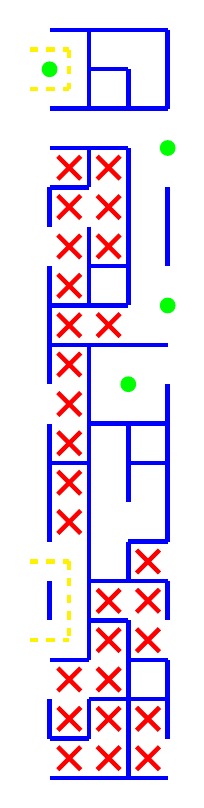
\begin{tikzpicture}[x=0.5cm, y=-0.5cm, ultra thick, blue]
% Walls
    \draw (0,0) -- (3,0);
    \draw (1,1) -- (2,1);
    \draw (0,2) -- (3,2);
    \draw (0,3) -- (2,3);
    \draw (0,4) -- (1,4);
    \draw (1,6) -- (2,6);
    \draw (0,7) -- (2,7);
    \draw (0,8) -- (3,8);
    \draw (1,10) -- (3,10);
    \draw (0,11) -- (1,11);
    \draw (2,11) -- (3,11);
    \draw (2,13) -- (3,13);
    \draw (1,14) -- (3,14);
    \draw (1,15) -- (2,15);
    \draw (0,16) -- (1,16);
    \draw (2,16) -- (3,16);
    \draw (1,17) -- (3,17);
    \draw (0,18) -- (1,18);
    \draw (0,19) -- (3,19);
    \draw (0,4) -- (0,5);
    \draw (0,6) -- (0,9);
    \draw (0,10) -- (0,13);
    \draw (0,14) -- (0,15);
    \draw (0,17) -- (0,18);
    \draw (1,0) -- (1,2);
    \draw (1,3) -- (1,4);
    \draw (1,5) -- (1,7);
    \draw (1,8) -- (1,16);
    \draw (1,17) -- (1,18);
    \draw (2,1) -- (2,2);
    \draw (2,3) -- (2,7);
    \draw (2,10) -- (2,12);
    \draw (2,13) -- (2,14);
    \draw (2,15) -- (2,19);
    \draw (3,0) -- (3,2);
    \draw (3,4) -- (3,6);
    \draw (3,9) -- (3,13);
    \draw (3,14) -- (3,15);
    \draw (3,16) -- (3,18);
% Pillars
    \fill[green] (0,1) circle(0.2);
    \fill[green] (3,3) circle(0.2);
    \fill[green] (3,7) circle(0.2);
    \fill[green] (2,9) circle(0.2);
% Inner points in accessible cul-de-sacs
    \node at (0.5,3.5) {};
    \node at (1.5,3.5) {};
    \node at (0.5,4.5) {};
    \node at (1.5,4.5) {};
    \node at (0.5,5.5) {};
    \node at (1.5,5.5) {};
    \node at (0.5,6.5) {};
    \node at (0.5,7.5) {};
    \node at (1.5,7.5) {};
    \node at (0.5,8.5) {};
    \node at (0.5,9.5) {};
    \node at (0.5,10.5) {};
    \node at (0.5,11.5) {};
    \node at (0.5,12.5) {};
    \node at (2.5,13.5) {};
    \node at (1.5,14.5) {};
    \node at (2.5,14.5) {};
    \node at (1.5,15.5) {};
    \node at (2.5,15.5) {};
    \node at (0.5,16.5) {};
    \node at (1.5,16.5) {};
    \node at (0.5,17.5) {};
    \node at (1.5,17.5) {};
    \node at (2.5,17.5) {};
    \node at (0.5,18.5) {};
    \node at (1.5,18.5) {};
    \node at (2.5,18.5) {};
% Entry-exit paths without intersections
    \draw[dashed, yellow] (-0.5,0.5) -- (0.5,0.5);
    \draw[dashed, yellow] (-0.5,1.5) -- (0.5,1.5);
    \draw[dashed, yellow] (-0.5,13.5) -- (0.5,13.5);
    \draw[dashed, yellow] (-0.5,15.5) -- (0.5,15.5);
    \draw[dashed, yellow] (0.5,0.5) -- (0.5,1.5);
    \draw[dashed, yellow] (0.5,13.5) -- (0.5,15.5);
\end{tikzpicture}
\end{center}
\vspace*{\fill}

\end{document}
